\documentclass{article}
%Packages
\usepackage{tikz}
\usetikzlibrary{shapes,arrows, positioning}


\begin{document}

\section{How to Draw Diamond in Latex}
  



\begin{tikzpicture}
	\node[diamond,draw]{Decision}; %For Diamond

\end{tikzpicture}

% If you want to change the width as well as vthe height of the diamond...use aspect
% Example 1
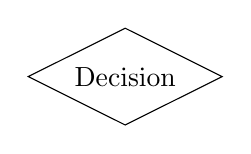
\begin{tikzpicture}
	\node[diamond,draw,aspect=2]{Decision}; % If you put aspect tool..you will see the lenght and the width will change.
\end{tikzpicture}

% Example 2
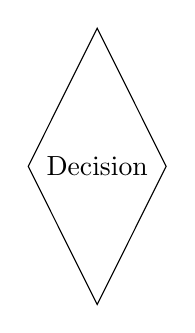
\begin{tikzpicture}
\node[diamond,draw,aspect=0.5]{Decision};
\end{tikzpicture}



\end{document}


